In this exercise, we will write two small computer programs for random
walks on a $2D$ square lattice:
\begin{itemize}
    \item one for the usual random walk, where the walker is allowed to 
        come back to points already visited
    \item one for the so-called self-avoiding random walk (SAW), 
        where the walker is not allowed to do so and hence does not 
        cross its own path.
\end{itemize}
HINT: One can find a lot of algorithms for the SAW in the web. It is ok 
to use just the simplest one: When the walker revisits a position, you 
discard the walk. Otherwise you use the trajectory. Note that this 
algorithm for the SAW is not very efficient (you have to reject more 
and more trajectories for larger $n$), so you should restrict yourself 
to $n<N$ with, say, $N=30$. For the usual random walk there is no such 
problem and you can explore larger $N$.

\paragraph{a) Write the program for a typical RW} \ \\
\\
    The code for a non-self-avoiding random walk is pretty 
    straight-forward: At each step, we randomly choose an axis along
    which we will move ($x$ or $y$), and then choose a random 
    number from the set $\{-1, +1\}$ to get the direction along the 
    chosen axis:
    $y$-direction, respectively. \\
    \begin{code}{calc\_random\_walk\_trajectory.py}
        import numpy as np
        
        
        def main(nr_of_steps, x=0, y=0):
        
            def random_step(x, y):
                direction = np.random.choice(['x', 'y'])
                if direction == 'x':
                    dx = np.random.choice([-1, 1])
                    dy = 0
                elif direction == 'y':
                    dx = 0
                    dy = np.random.choice([-1, 1])
        
            trajectory = []
            for i in range(nr_of_steps):
                x, y = random_step(x, y) 
                trajectory.append((x, y))
        
            return trajectory\end{code} \ \\
    \noindent
    It was not entirely clear from the formulation in the problem set 
    whether diagonal steps are allowed as well. 
    Including them would lead to the step size not being constant 
    (sometimes being $1$, sometimes $\sqrt{2}$). If one wishes to 
    allow diagonal steps as well, one could simply adjust the 
    \lstinline{random_step} method like this: \\
    \begin{code}{calc\_random\_walk\_trajectory.py}
        def random_step(x, y):
            dx = np.random.choice([-1, 0, 1])
            dy = np.random.choice([-1, 0, 1])
            return x+dx, y+dy\end{code}

\newpage
\paragraph{b) Write the program for a SAW} \ \\
\\
    To make the random walk self-avoiding, we simply have to check 
    at each step whether or not the position of the next step has 
    already been reached at an earlier time. If it has, we just return 
    \lstinline{None} instead of the trajectory. Outside of
    \lstinline{calc_random_walk_trajectory} in the 
    \lstinline{main} function, we run a 
    \lstinline{while} loop, which repeats the function execution until a 
    non-\lstinline{None} value has been returned.
    \begin{code}{calc\_random\_walk\_trajectory.py}
        import numpy as np
        
        
        def main(nr_of_steps, self_avoiding=True, x=0, y=0):
        
            def random_step(x, y):
                direction = np.random.choice(['x', 'y'])
                if direction == 'x':
                    dx = np.random.choice([-1, 1])
                    dy = 0
                elif direction == 'y':
                    dx = 0
                    dy = np.random.choice([-1, 1])
                return x+dx, y+dy

            trajectory = []
            for i in range(nr_of_steps):
                x, y = random_step(x, y)
        
                if self_avoiding and (x, y) in trajectory:
                    return None
        
                trajectory.append((x, y))
        
            return trajectory\end{code}

    \begin{code}{main.py}
        from calc_random_walk_trajectory import main as calc_random_walk_trajectory
        
        
        def main(nr_of_steps=30, self_avoiding=True):
        
            trajectory = calc_random_walk_trajectory(nr_of_steps, self_avoiding)
            if self_avoiding:
                while trajectory is None:
                    trajectory = calc_random_walk_trajectory(
                        nr_of_steps, self_avoiding
                    )
        
            filename = 'SAW' if self_avoiding else 'RW'
            plot_trajectory(trajectory, nr_of_steps, filename)\end{code}

\newpage
\paragraph{c) Show some representative trajectories.} \ \\
\\
    Without diagonal steps:
    \begin{figure}[h!]
        \centering
        \begin{minipage}{.5\linewidth}
          \centering
          \subfloat[normal random walk ($n=400$)]{
            \label{:a}
            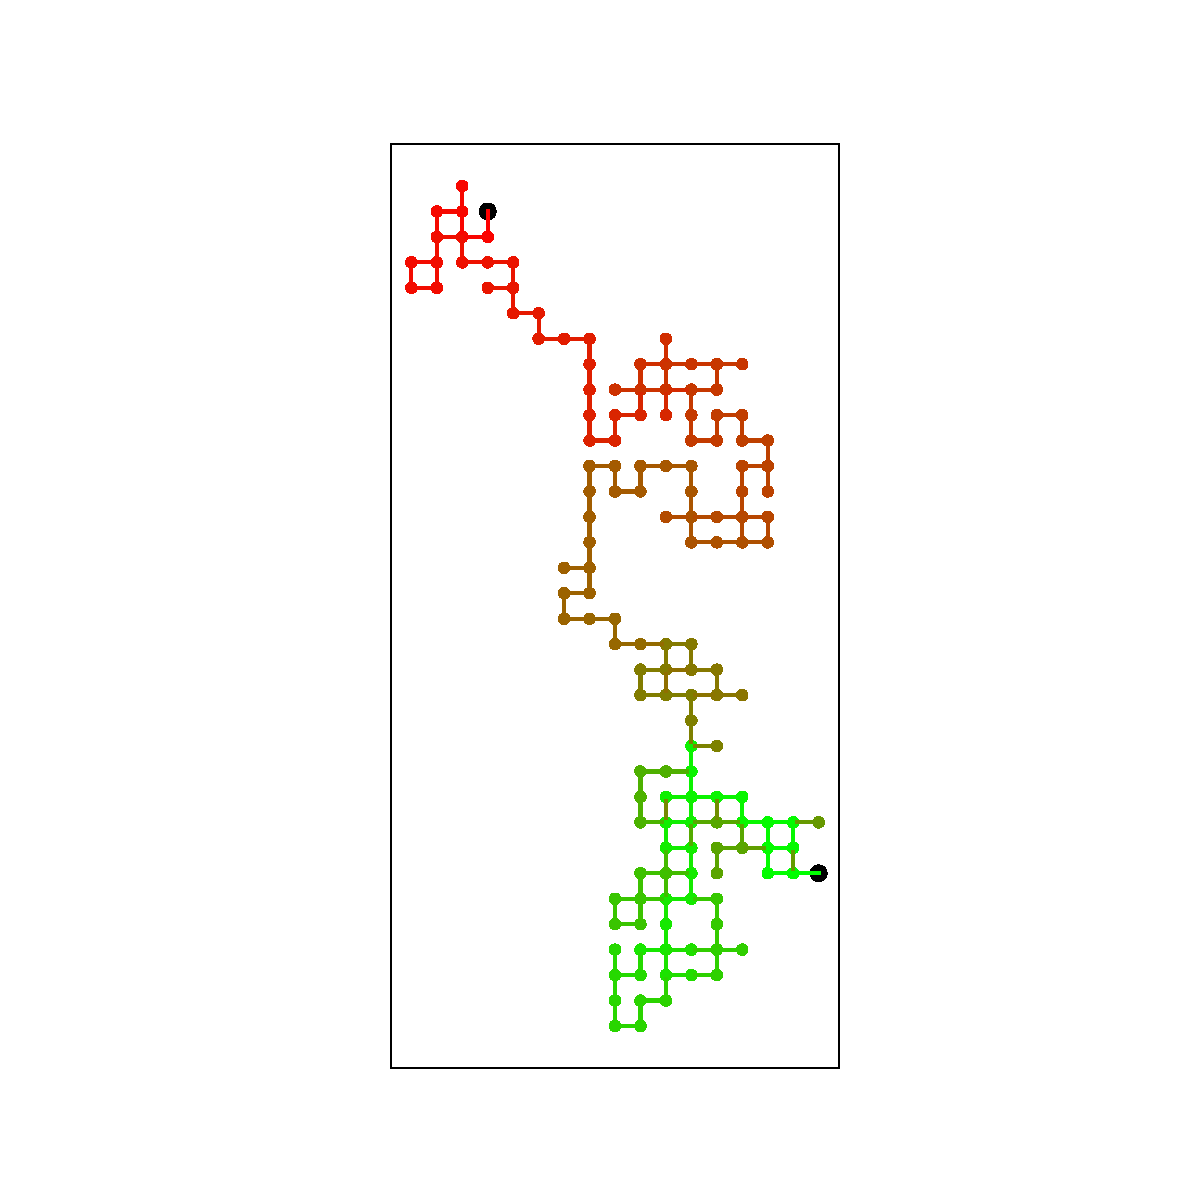
\includegraphics[scale=.45]{./figures/RW.pdf}
            % 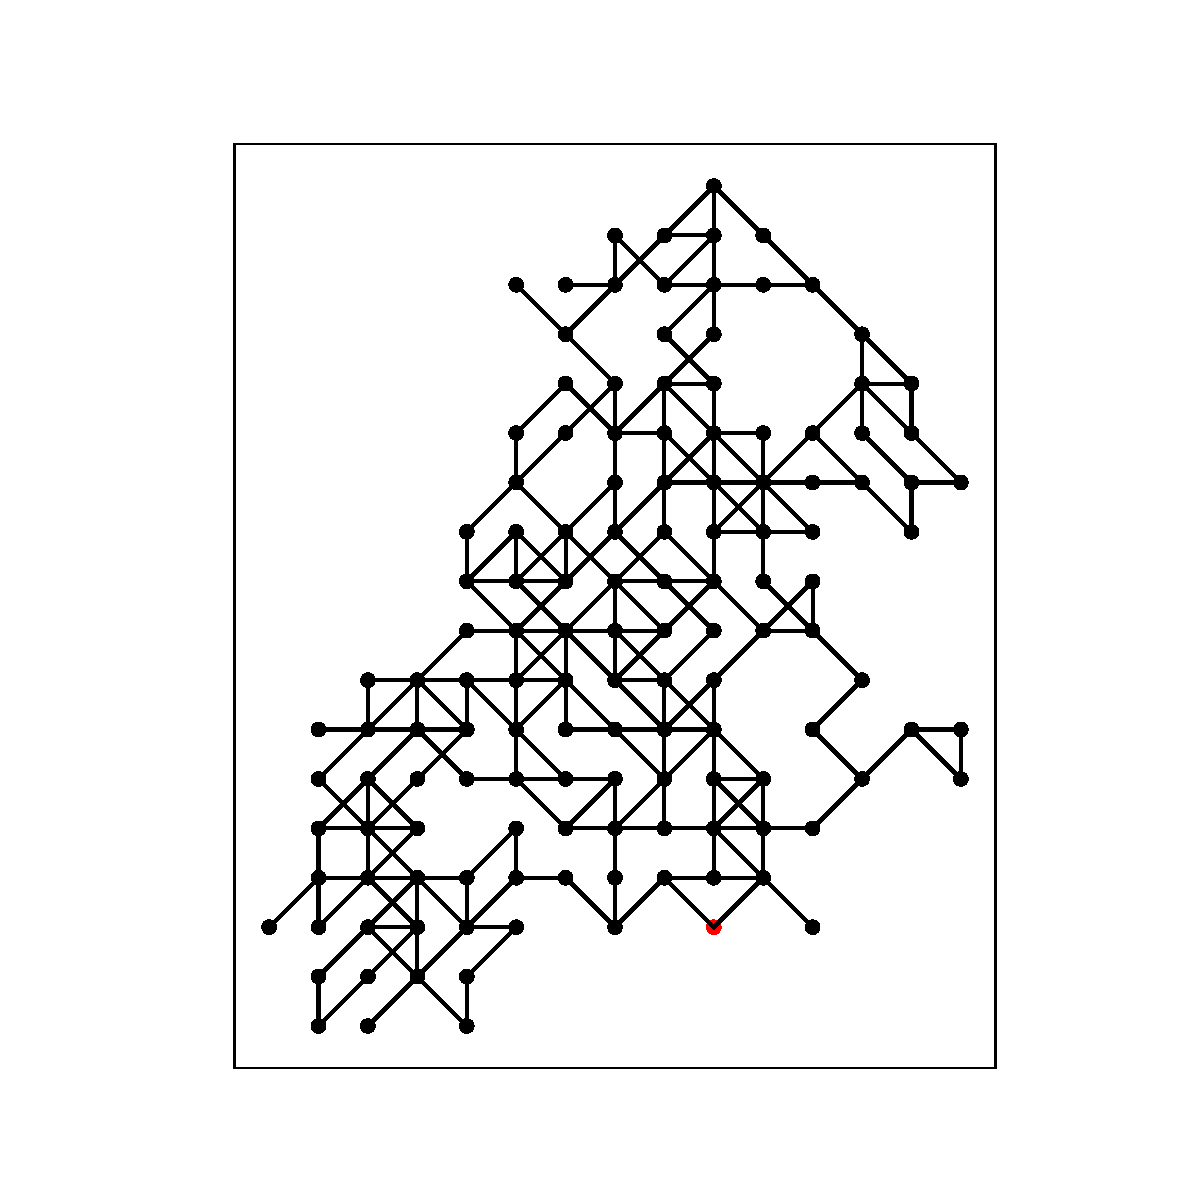
\includegraphics[scale=.5]{./figures/RW_good.pdf}
          }
        \end{minipage}%
        \begin{minipage}{.5\linewidth}
          \centering
          \subfloat[self-avoiding random walk ($n=30$)]{
            \label{:b}
            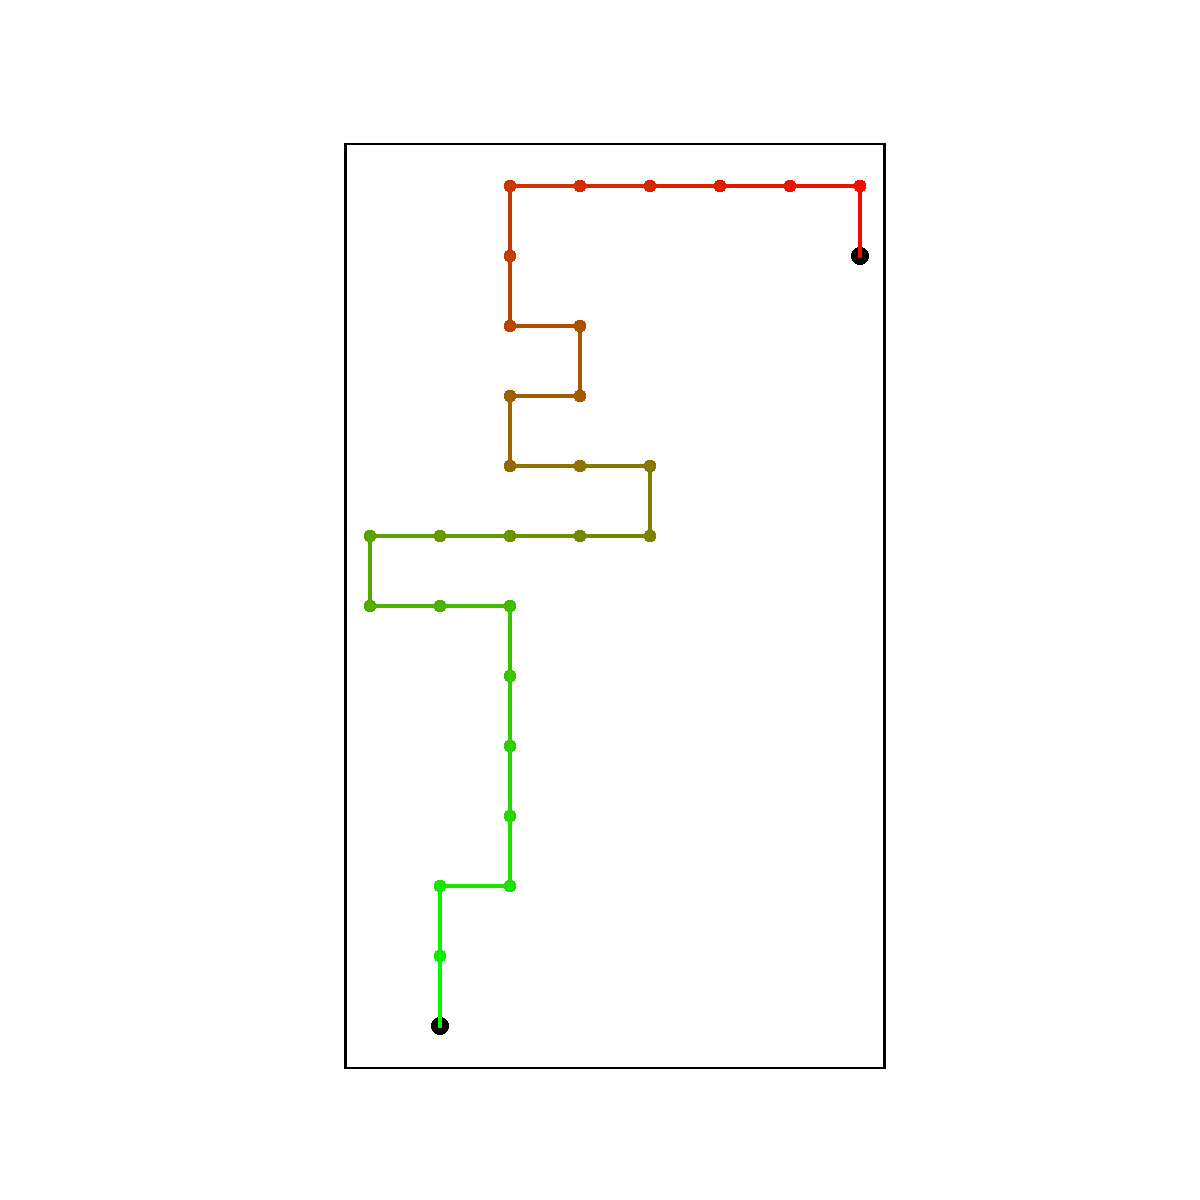
\includegraphics[scale=.45]{./figures/SAW.pdf}
            % 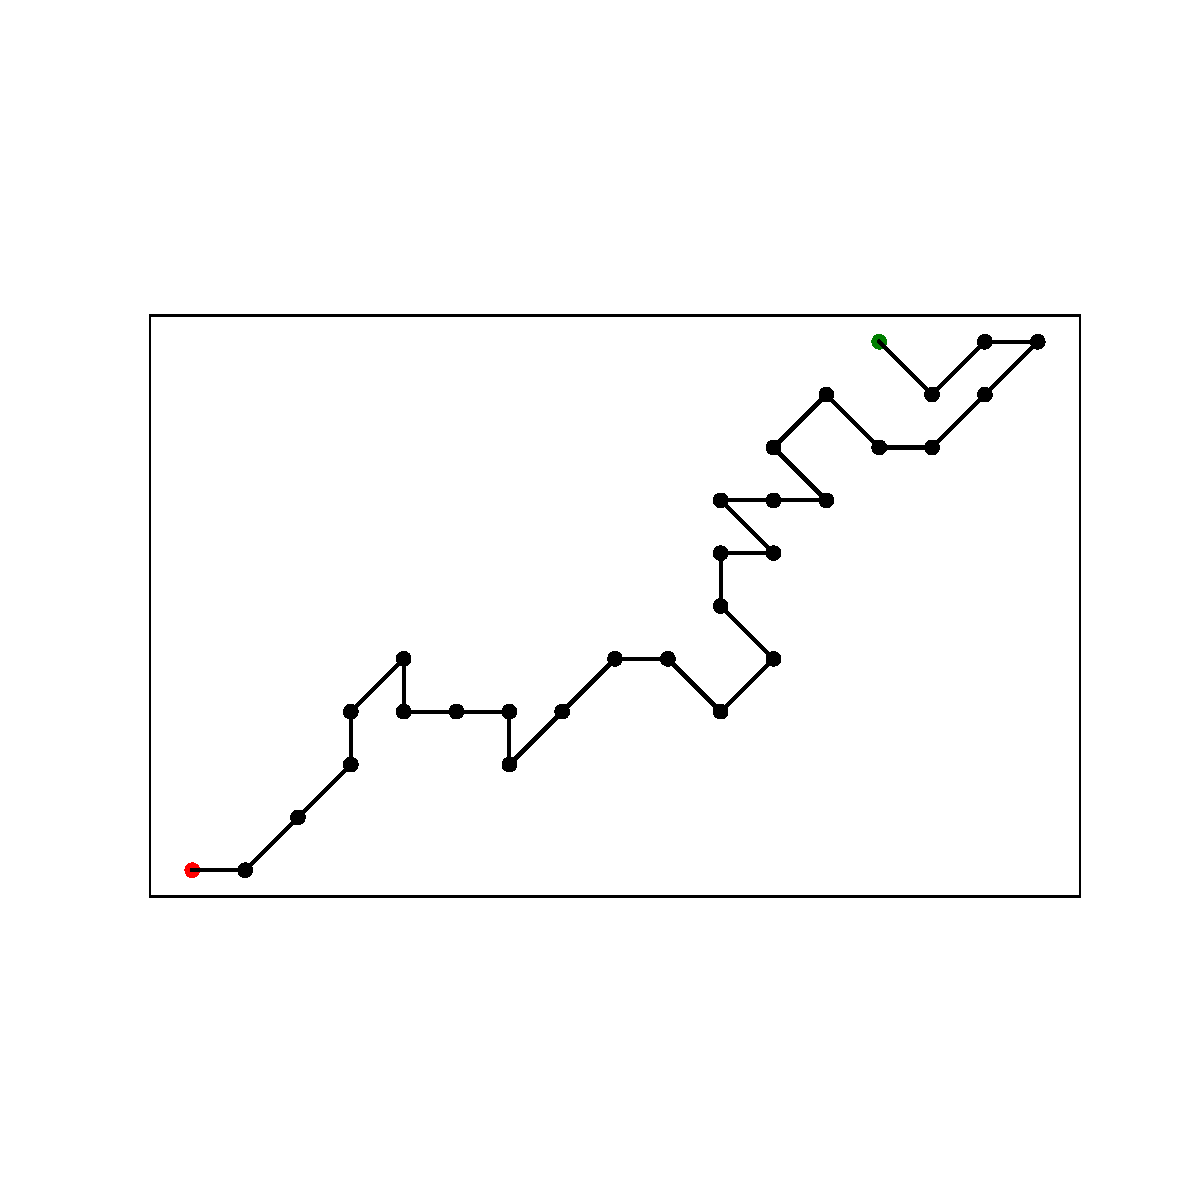
\includegraphics[scale=.5]{./figures/SAW_good.pdf}
          }
        \end{minipage}
    \end{figure} \ \\
    With diagonal steps:
    \begin{figure}[h!]
        \centering
        \begin{minipage}{.5\linewidth}
          \centering
          \subfloat[normal random walk ($n=400$)]{
            \label{:a}
            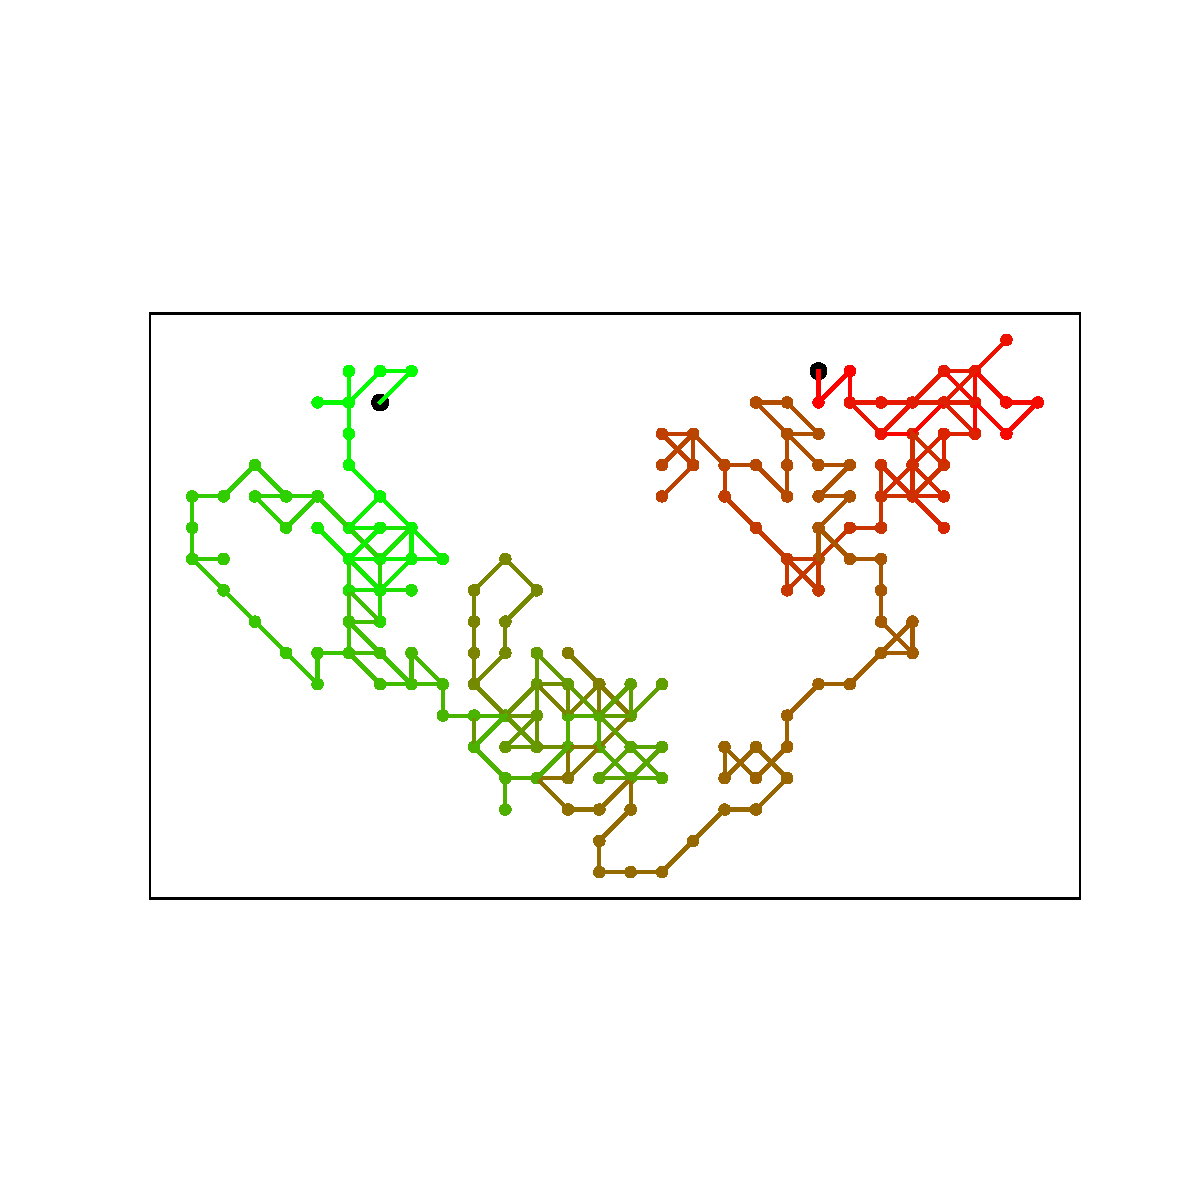
\includegraphics[scale=.45]{./figures/RW_diag.pdf}
            % 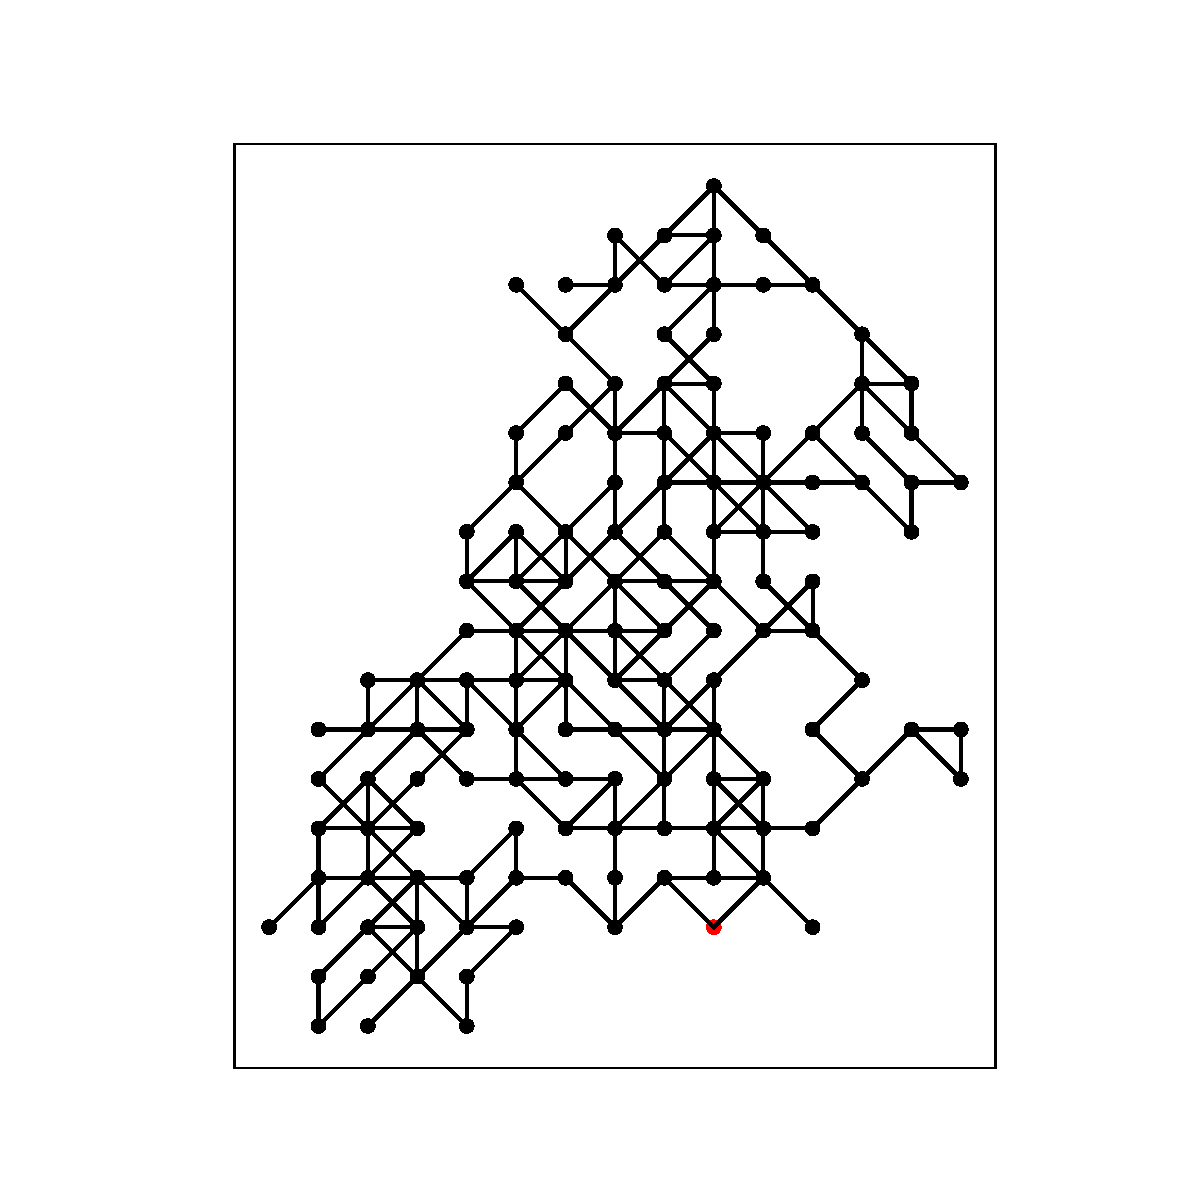
\includegraphics[scale=.5]{./figures/RW_good.pdf}
          }
        \end{minipage}%
        \begin{minipage}{.5\linewidth}
          \centering
          \subfloat[self-avoiding random walk ($n=30$)]{
            \label{:b}
            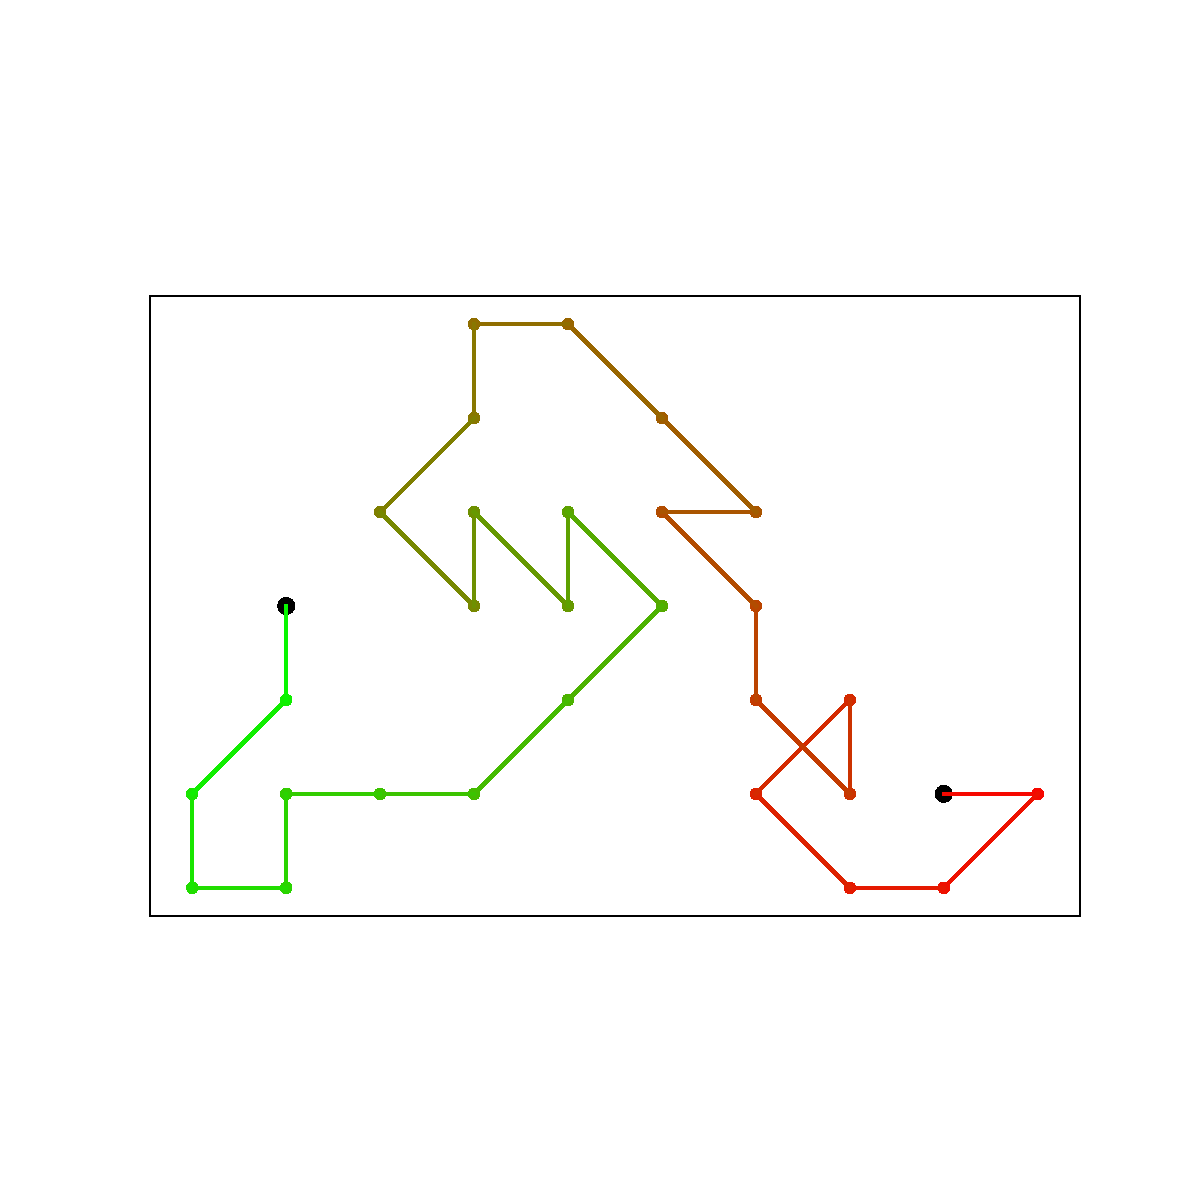
\includegraphics[scale=.45]{./figures/SAW_diag.pdf}
            % 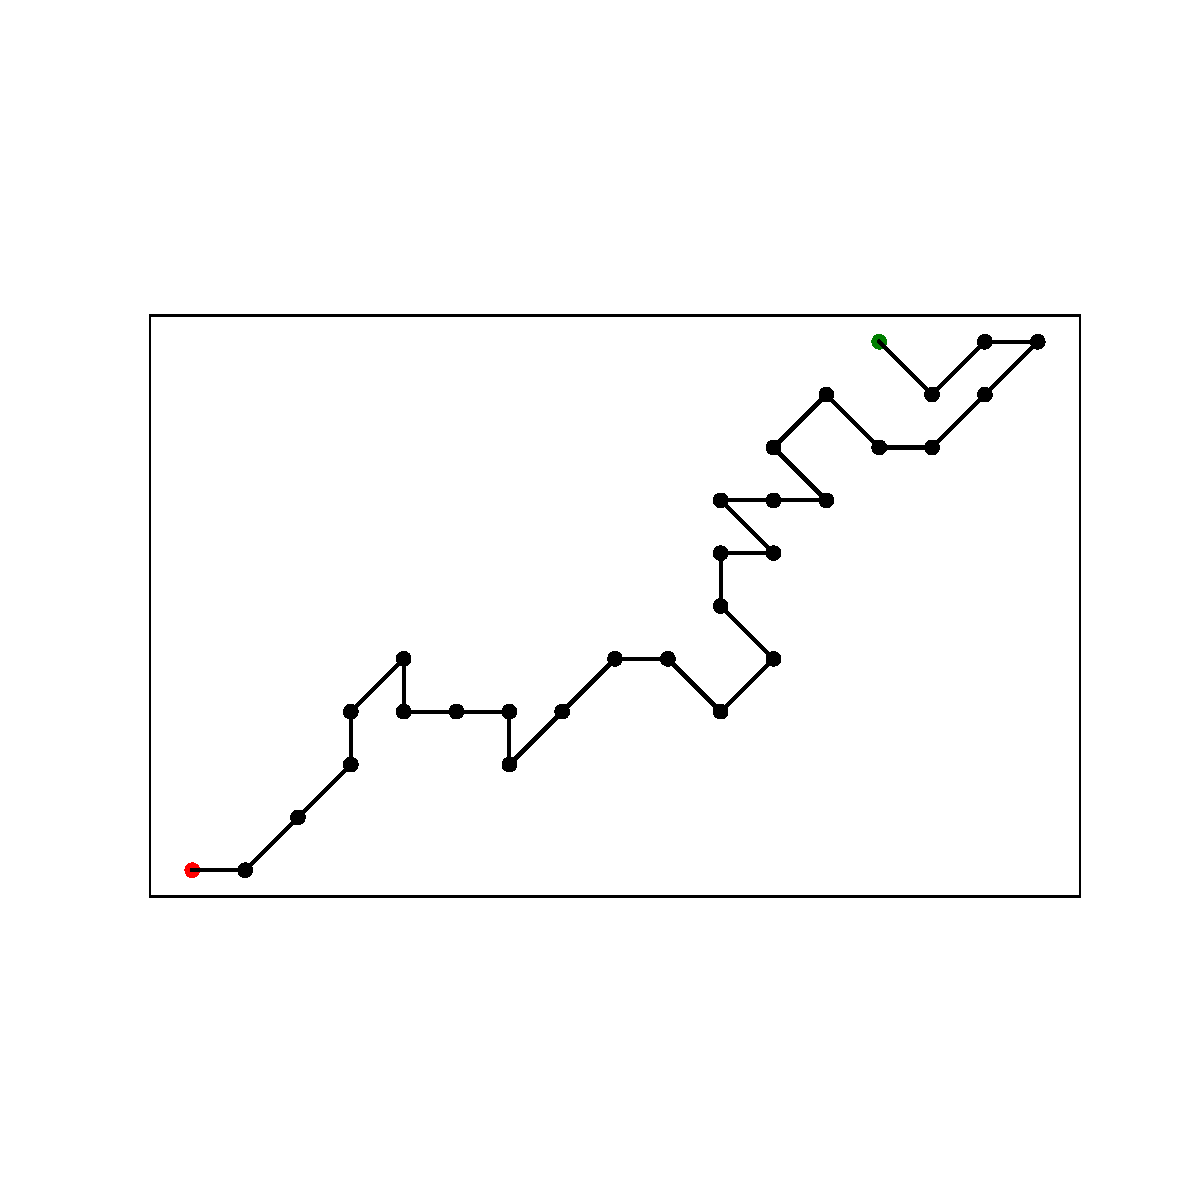
\includegraphics[scale=.5]{./figures/SAW_good.pdf}
          } 
        \end{minipage}
    \end{figure} \ \\
    When the particle crosses its own path, the trajectory can
    look a bit messy. Therefore, we added a color coding from 
    green (first step) to red (last step) to improve the 
    visualization.

\newpage
\paragraph{d) Measure the mean squared displacements (MSD) 
    $\langle x^2(n)\rangle$ as a function of the number of steps $n$ 
    for both cases (the average is over different trajectories). If you 
    plot the results in log-log-scale you can extract the exponents 
    $\alpha$, where $\langle x^2(n)\rangle\sim n^\alpha$, for the two 
    cases. Compare and discuss.
} \ \\
\\
    To get the average over different trajectories, for each number of 
    steps we calculate 100 trajectories (in this case, without 
    allowing diagonal steps), then we calculate the squared 
    displacements for each of the trajectories and take the mean.
    Then, we plot this in a linear fashion: \\
    % \begin{figure}[h!]
    %     \centering
    %     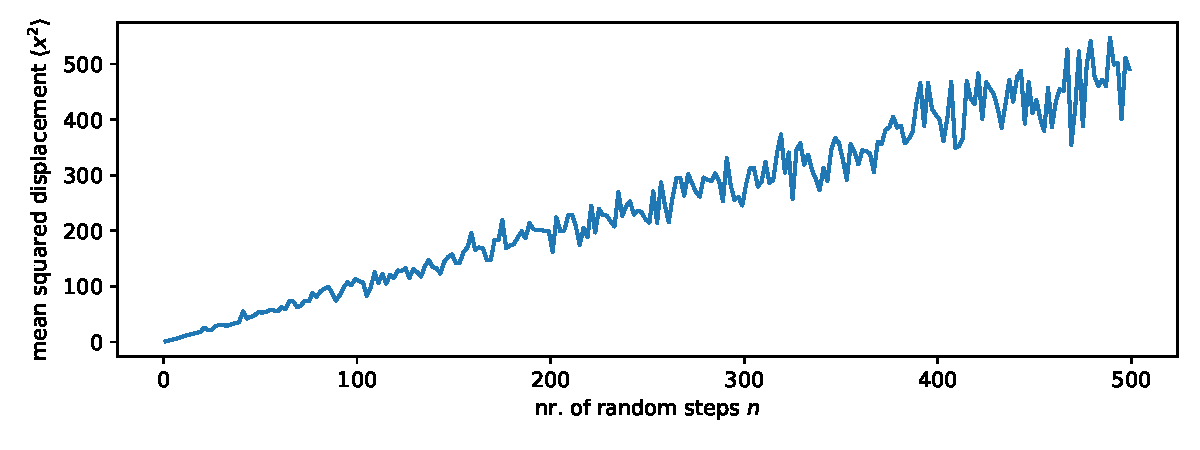
\includegraphics[width=\textwidth]{./figures/MSD_vs_N.pdf}
    %     \caption{mean squared displacement as a function of steps}
    % \end{figure} \ \\
    \begin{figure}[h!]
        \centering
        \begin{minipage}{.5\linewidth}
          \centering
          \subfloat[linear plot for the normal RW]{
            \label{:a}
            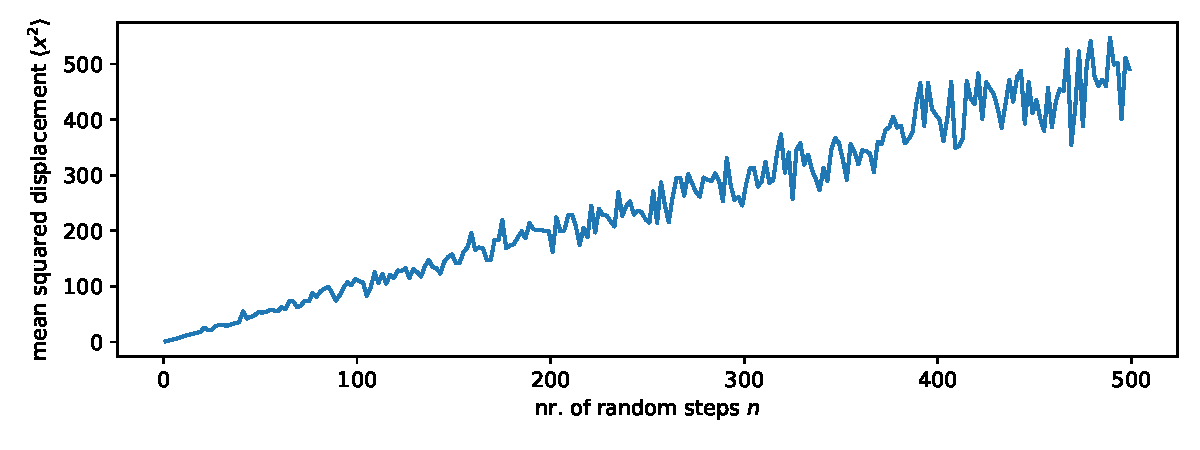
\includegraphics[scale=.7]{./figures/MSD_vs_N.pdf}
          }
        \end{minipage}%
        \begin{minipage}{.5\linewidth}
          \centering
          \subfloat[linear plot for the SAW]{
            \label{:b}
            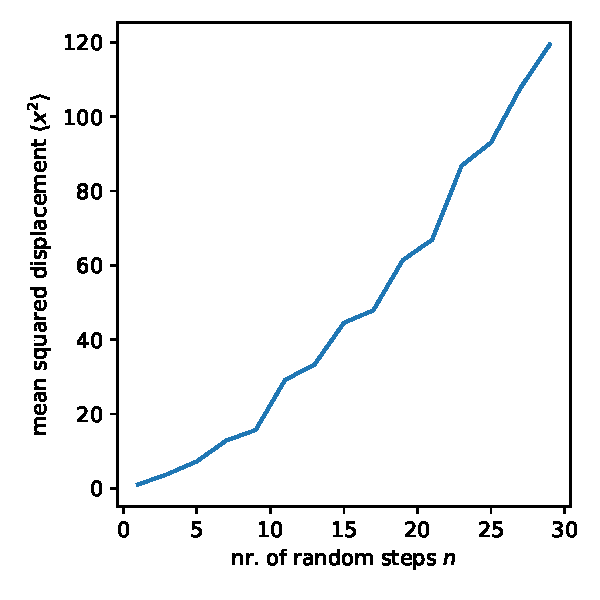
\includegraphics[scale=.7]{./figures/MSD_vs_N_SA.pdf}
          }
        \end{minipage}
    \end{figure} \ \\
    And now as a log-log plot: \\
    % \begin{figure}[h!]
    %     \centering
    %     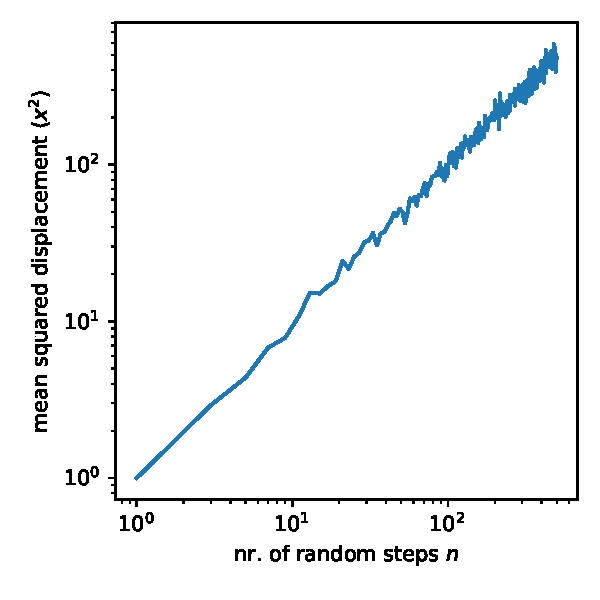
\includegraphics[width=\textwidth]{./figures/MSD_vs_N_loglog.pdf}
    %     \caption{mean squared displacement as a function of steps}
    % \end{figure} \ \\
    \begin{figure}[h!]
        \centering
        \begin{minipage}{.5\linewidth}
          \centering
          \subfloat[log-log plot for the normal RW]{
            \label{:a}
            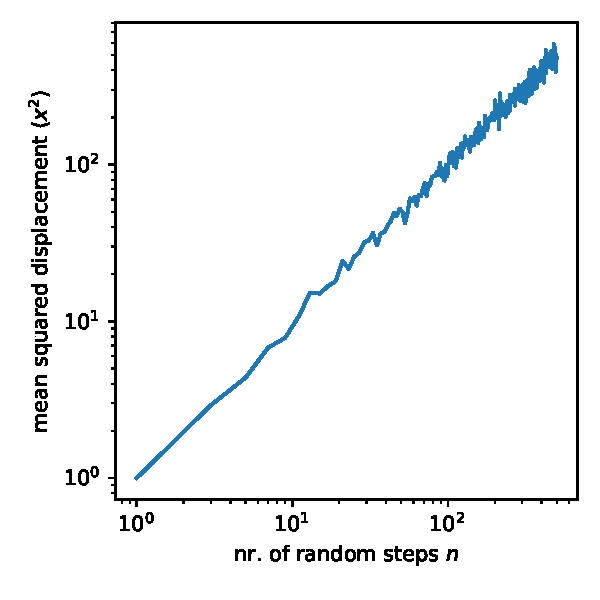
\includegraphics[scale=.7]{./figures/MSD_vs_N_loglog.pdf}
          }
        \end{minipage}%
        \begin{minipage}{.5\linewidth}
          \centering
          \subfloat[log-log plot for the SAW]{
            \label{:b}
            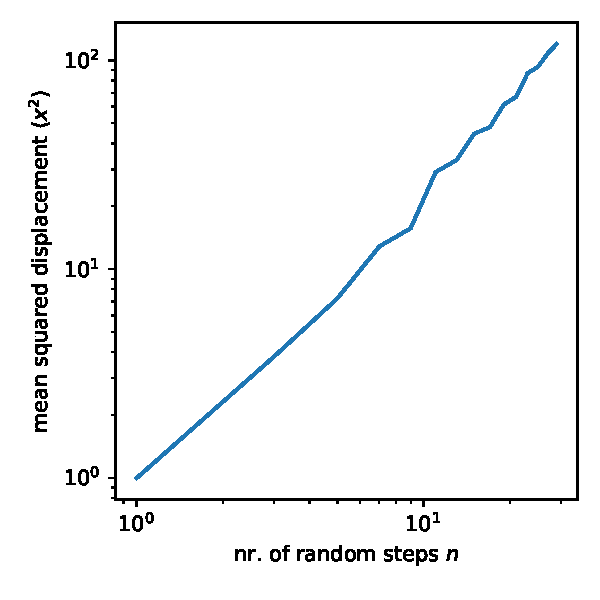
\includegraphics[scale=.7]{./figures/MSD_vs_N_loglog_SA.pdf}
          }
        \end{minipage}
    \end{figure} \ \\
    \\
    As expected, we find $\alpha\approx1$ for the normal 
    random-walk. The self-avoiding random walk leads to an 
    exponent of $\alpha>1$, which also makes sense, since the 
    movement of the particle is restricted in a way that makes 
    it less likely to travel towards its point of origin.
